\documentclass{report}

\usepackage[margin=1.5cm]{geometry}
\usepackage{hyperref}
\usepackage{graphicx}

\graphicspath{ {./img/} }

\author{Blascovich Alessio\\ 217317\\ \href{mailto:alessio.blascovich@studenti.unitn.it}{alessio.blascovich@studenti.unitn.it}}
\title{Sistemi informativi\\ Secondo assignement}
\date{}

\begin{document}
   \maketitle

   \begin{abstract}
      Creare un modello a stella per il fatto "ordini" a partire dallo schema di base di dati allegato (NorthWind), identificando le misure e le dimensioni (con eventuale gerarchia) che si vogliono associare al fatto principale (gli ordini).
      \begin{center}
         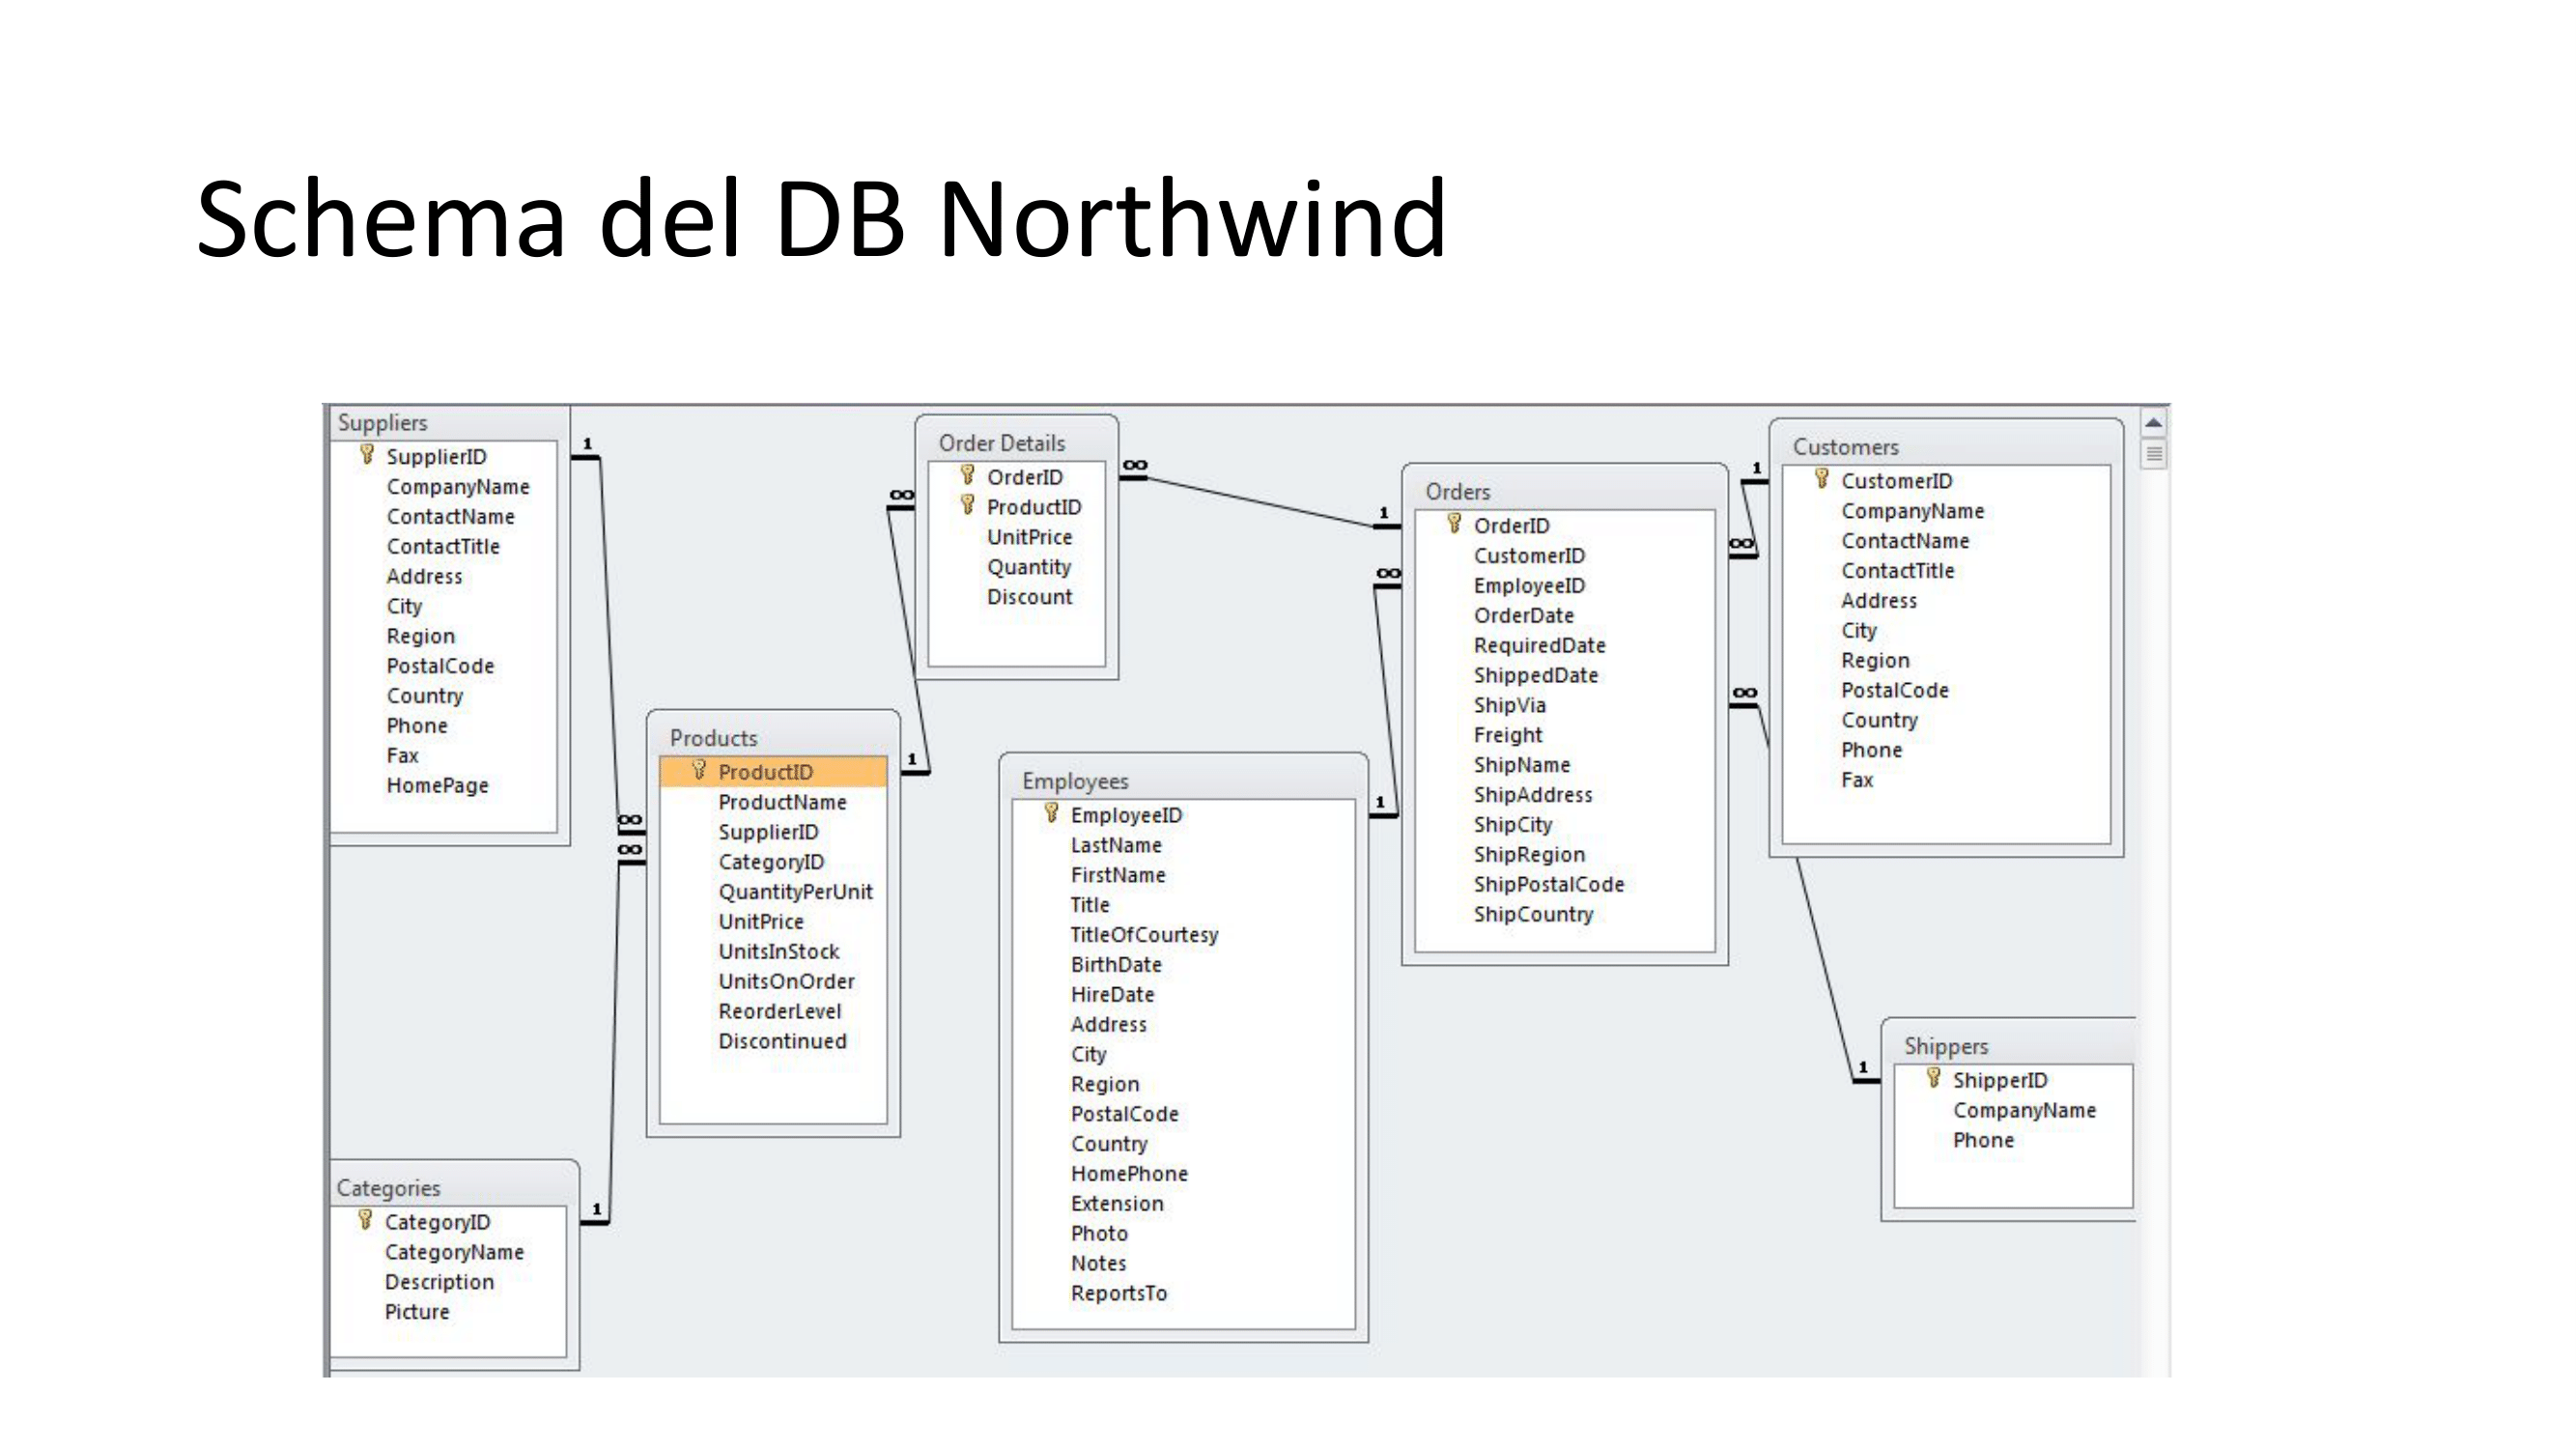
\includegraphics[scale=0.5]{testo_assignement.png}
      \end{center}
   \end{abstract}

   \chapter*{Schema a stella}
   \begin{center}
      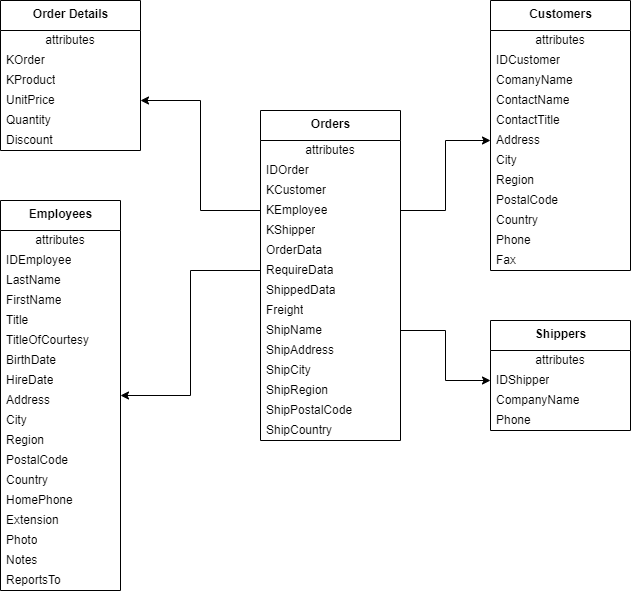
\includegraphics[scale=0.7]{Assignement2.png}
   \end{center}
\end{document}